\subsection{Centralized Similarity Join}
\label{sec:centralized}

A na\"ive approach to answer a hybrid similarity join query over two geolocated time series $\mathcal{T}_{R}, \mathcal{T}_{S}$ would involve examination of all possible pairs, i.e., calculating their Cartesian product $\mathcal{T}_{R} \times \mathcal{T}_{S}$ and filtering each candidate pair with the two criteria. Clearly, such a technique has limitations due to its quadratic processing cost and cannot be realistically applied against datasets with more than a few thousand objects each.  
Hence, we propose three {\em index-based} techniques for answering hybrid similarity join queries:

\begin{itemize}
\item We describe a {\em spatial-only} filtering method that employs R-trees over the locations of objects so as to identify candidate pairs close enough in space. Afterwards, the time series of each such candidate pair should also be checked on their similarity to finally yield the exact answer (Section~\ref{subsec:rtree}). 
\item We build \isax indices {\em over the time series} information only per dataset and we introduce a traversal method to facilitate similarity search. Refinement over returned candidate pairs by their spatial distance issues the final results (Section~\ref{subsec:isax_appr}).
\item We employ {\btsr}s that can {\em jointly} index the positional and time series information of each object.  We introduce a {\em hybrid similarity join} algorithm that descends these two BTSR-trees in tandem and can safely prune subtrees that cannot possibly contribute any valid results (Section~\ref{subsec:btsr_appr}).
\end{itemize}

In each of these methods, one global index is created per dataset. Hence, a {\em centralized} processor is responsible to maintain these indices and access them when evaluating similarity join queries.


\subsubsection{Spatial-Only Filtering using R-Trees}
\label{subsec:rtree}

One possible approach to similarity join search over two datasets $\mathcal{T}_{R}, \mathcal{T}_{S}$ of geolocated time series is to build an R-tree \cite{Guttman1984} per dataset by organizing its spatial locations into a hierarchy of nested $d$-dimensional rectangles. Each node corresponds to a disk page and represents the MBR of its children. A leaf holds the MBR of its contained geometries. The number of entries per node (excluding the root) is between a lower bound $m$ and a maximum capacity $M$.

With respect to {\em hybrid similarity joins}, we search over R-trees using the spatial condition, exactly as in \cite{DBLP:conf/sigmod/BrinkhoffKS93}. So, both R-trees are concurrently traversed starting from their roots and recursively examining their respective descendants only if the minimum distance $MINDIST$ of their MBRs \cite{DBLP:conf/sigmod/RoussopoulosKV95} does not exceed parameter $\epsilon_{sp}$. Obviously, a pair of nodes breaking this spatial constraint cannot possibly contain any qualifying results, so their respective subtrees can be safely pruned. Once the leaf levels are reached, the candidate pairs of raw time series are accessed and refined according to both criteria in Definition~\ref{def:sim_join} in order to issue the final results. 
 


\subsubsection{Time Series-Only Filtering with iSAX}
\label{subsec:isax_appr}

This method makes use of available \isax indices over two datasets $\mathcal{T}_{R}, \mathcal{T}_{S}$, each concerning their respective time series as discussed in Section~\ref{subsec:isax}. Each \isax index solely indexes the time series part of a dataset; their leaf entries point to the raw time series including their location. Searching for similar objects starts from the root of each tree and progressively descends by visiting nodes that may contain candidate answers based on their similarity, strictly on the time series domain, as listed in Algorithm~\ref{alg:sim_joins_isax}. Without loss of generality, we assume that either the trees have the same height, or the \isax for $\mathcal{T}_{R}$ is less deep than the \isax for $\mathcal{T}_{S}$.

Suppose that at a given iteration, node $R$ in the first \isax needs to be checked against node $S$ in the second \isax. If neither of them is leaf, the algorithm is recursively called against all combinations of their children entries, provided that these are within distance $\epsilon_{ts}$ as computed by Eq.~\ref{eq:dist_ts} (Lines 1-5). Once the leaf level is reached in the first \isax but not yet in the second \isax (if they differ in height), recursive calls examine that specific leaf of the former against each of the children entries of the latter (Lines 6-8).

%Note that \isax nodes actually index SAX words, hence these must be converted back to their PAA representation of time series in order to become comparable according to the distance measure specified in Eq.~\ref{eq:dist_ts}. \mnote{Does distance over PAAs can be used as a lower bound? In \cite{jessica2007dmkd}, it is proven that distance between PAAs lower bounds the Euclidean distance over the respective raw time series. As Euclidean distance can never exceed $d_{ts}$ as computed via Eq.~\ref{eq:dist_ts}, it seems that our filtering is safe. Distance $d_{SAX}$ from Eq.~\ref{eq:dist_sax} over their respective $SAX$ words is not actually used in filtering, but only in the construction of \isax indices.} %As $d_{SAX}$ is a lower bound on the Euclidean distance between all time series in the respective subtrees, this criterion guarantees no false misses.

Eventually, when the leaf level is reached in both trees, we compare each combination of their respective contents (Lines 9-13). Each geolocated time series from leaf $R$ of the first \isax is checked with its counterparts in leaf $S$ of the second \isax. Since raw time series data is fully accessible at the leaf level (including locations), refinement of candidates is based not only on their distance $d_{ts}$ in the time series domain, but also on their spatial distance $d_{sp}$. If both distances are below the respective constraints, then this specific pair qualifies for the final result $Q$ to the query. The algorithm terminates once there are no remaining pairs of leaves to check.


\begin{algorithm}[!ht]
\begin{small}
	\DontPrintSemicolon
	\KwIn{Nodes $R$, $S$, spatial constraint $\epsilon_{sp}$, time series constraint $\epsilon_{ts}$}
	\KwOut{Set $Q$ of pairs of geolocated time series satisfying constraints}
	\BlankLine
	\If(\com*[f]{internal nodes in both trees}){$R$ is not leaf $\land \ S$ is not leaf}{
		\ForEach{$N_{R} \in R.getChildren()$}{
			\ForEach{$N_{S} \in S.getChildren()$}{
				\If(\com*[f]{compare SAX words}){$d_{SAX}(N_{R}, N_{S}) \leq \epsilon_{ts}$}{
					$SimJoinSAX(N_{R}, N_{S}, \epsilon_{sp}, \epsilon_{ts})$
				}
			}
		}
	}
	\ElseIf(\com*[f]{trees of different height}){$R$ is leaf $\land$ $S$ is not leaf}{
		\ForEach{$N_{S} \in S.getChildren()$}{
			$SimJoinSAX(R, N_{S}, \epsilon_{sp}, \epsilon_{ts})$
		}
	}

	\ElseIf(\com*[f]{leaf level in both trees}){$R$ is leaf $\land$ \  $S$ is leaf}{
		\ForEach{$T_{R} \in R.getChildren()$}{
			\ForEach{$T_{S} \in S.getChildren()$}{
				\If{$d_{sp}(T_{R}, T_{S})~\leq~\epsilon_{sp} \land d_{ts}(T_{R}, T_{S}) \leq \epsilon_{ts}$} {
					$Q \leftarrow Q \cup \{ (T_{R}, T_{S}) \}$ \com*[f]{add pair to result set}
				}
			}
		}
	}
	\caption{$SimJoinSAX(R, S, \epsilon_{sp}, \epsilon_{ts})$}
	\label{alg:sim_joins_isax}
\end{small}		
\end{algorithm}





\subsubsection{Hybrid Filtering using BTSR-Trees}
\label{subsec:btsr_appr}

This method makes use of a hybrid \btsr index per dataset $\mathcal{T}_{R}, \mathcal{T}_{S}$ of geolocated time series. Initially, let us assume that both {\btsr}s have the same height. Exactly like the  \isax-based method, search starts from the root of each tree and descends them in tandem by checking their nodes pairwise, as listed in Algorithm~\ref{alg:sim_joins_btsr}.

%As listed in Algorithm~\ref{alg:sim_joins_btsr}, suppose that node $R$ in the \btsr over dataset $\mathcal{T}_{R}$ needs to be checked against node $S$ in the \btsr for dataset $\mathcal{T}_{S}$. 

In case that the currently examined entries $R$ and $S$ are internal (directory) nodes, a nested-loop check finds which of their descendants may contain candidate results (Lines 1-6). In particular, for each child entry $N_R$ of node $R$, we calculate a buffer rectangle by expanding its respective MBR by distance $\epsilon_{sp}$. In case that this buffer intersects with the MBR of entry $N_S$ from node $S$, whereas also their MBTS do not deviate by more than $\epsilon_{ts}$, then search should be recursively applied against those two entries $N_R, N_S$. Clearly, if neither of these criteria is met, those candidate entries cannot possibly contain any matching time series. 




Note that this step involves comparison between two MBTSs. Consider two MBTSs $B_1 = (B_1^{\sqcup}, B_1^{\sqcap})$ and $B_2 = (B_2^{\sqcup}, B_2^{\sqcap})$, each constructed according to Eq.~\ref{eq:bounds1} over two disjoint subsets of time series data. We compute their {\em deviation} $d_{MBTS}$ by first comparing the lower bounding time series of the former with the upper bounding time series of the latter per time point $i \in \{ 1, \dots, n \}$, depending on which of these two values is larger, i.e.:
\begin{equation}
 \begin{split}
  \delta_i = \begin{cases}
	B_1^{\sqcup}.v_i - B_2^{\sqcap}.v_i, & \text{if} \;\; B_1^{\sqcup}.v_i \geq B_2^{\sqcap}.v_i \\
	B_2^{\sqcup}.v_i - B_1^{\sqcap}.v_i, & \text{if} \;\; B_2^{\sqcup}.v_i \geq B_1^{\sqcap}.v_i \\
	0, & \text{otherwise}
	  \end{cases}
 \end{split}
 \label{eq:delta_timepoint}
\end{equation}
\noindent and we take the average Euclidean norm over these $n$ differences:
\begin{equation} \label{eq:dist_mbts}
d_{MBTS}(B_1, B_2) = \frac{1}{n}\sqrt{\displaystyle \sum_{i=1}^{n}({\delta}_i)^2}
\end{equation}
Quite importantly, this measure is a {\em lower bound} of the Euclidean distance $d_{ts}(T_1, T_2)$  between two time series $T_1, T_2$ that are enclosed in MBTSs $B_1, B_2$, respectively. Consider the situation at a given time point $i \in \{ 1, \dots, n \}$. In case that $B_1^{\sqcup}.v_i \geq B_2^{\sqcap}.v_i$, it is straighforward that $T_1.v_i \geq B_1^{\sqcup}.v_i \geq B_2^{\sqcap}.v_i \geq T_2.v_i$ by definition of the MBTS, hence ${\delta}'_i = T_1.v_i - T_2.v_i \geq {\delta}_i$. This also holds for the other branches of Eq.~\ref{eq:delta_timepoint}. But, taking the Euclidean norm of these ${\delta}'_i$ values over all time points expresses the time series similarity according to Eq.~\ref{eq:dist_ts}. Overall, this confirms that $d_{ts}(T_1, T_2) \geq d_{MBTS}(B_1, B_2)$, so checking with MBTSs does not cause any false misses.
   

                              
\eat{   

Since each of these bounds is actually a time series, this computation is based on Eq.~\ref{eq:dist_ts} as follows:
\begin{equation} \label{eq:dist_mbts}
d_{MBTS}(B_1, B_2) =  \max ( d_{ts}(T_1^{\sqcup}, T_2^{\sqcap}), d_{ts}(T_2^{\sqcup}, T_1^{\sqcap}) ).
\end{equation}
\noindent Essentially, this distance measure captures the maximum possible deviation across sequence length $n$ between any of the time series contained in one MBTS with those contained in the other one. If this distance exceeds a given value $\epsilon_{ts}$, there is no possibility of finding any pair of similar time series between the two MBTS.

\mnote{Alternative formula reflecting what is essentially used in the implementation. Which one is  correct?}
\begin{equation} \label{eq:dist_mbts2}
d_{MBTS}(B_1, B_2) =  \max \{ \max (T_1^{\sqcup}.v_i - T_2^{\sqcap}.v_i, T_2^{\sqcup}.v_i - T_1^{\sqcap}.v_i) : i = 1..n \}.
\end{equation}


\mnote{It can be proven that distance $d_{MBTS}$ is an upper bound ??? over the distance of any pair of time series coming from those two MBTS.}

}



If both $R$ and $S$ are leaves, the algorithm retrieves all time series from either leaf and checks every combination against both criteria (Lines 10-14). If a time series from $\mathcal{T}_{R}$ and a time series from $\mathcal{T}_{S}$ are close enough in space (i.e., less than $\epsilon_{sp}$) and also similar in the time series domain by $\epsilon_{ts}$, this pair is issued as result.



\begin{algorithm}[!ht]
\begin{small}
	\DontPrintSemicolon
	\KwIn{Nodes $R$, $S$, spatial constraint $\epsilon_{sp}$, time series constraint $\epsilon_{ts}$}
	\KwOut{Set $Q$ of pairs of geolocated time series satisfying constraints}
	\BlankLine
	\uIf(\com*[f]{internal nodes in both trees}){$R$ is not leaf $\land \ S$ is not leaf}{
		\ForEach{$N_{R} \in R.getChildren()$}{
			$N_{R}.buf \leftarrow buffer(N_{R}.mbr, \epsilon_{sp})$ \com*[f]{expand MBR by $\epsilon_{sp}$} \\
			\ForEach{$N_{S} \in S.getChildren$}{
				\If{$N_{R}.buf \cap N_{S}.mbr \neq \emptyset \land d_{MBTS}(N_{R}, N_{S}) \leq \epsilon_{ts}$}{
					$SimJoinBTSR(N_{R}, N_{S}, \epsilon_{sp}, \epsilon_{ts})$
				}
			}
		}
	}
	\uElseIf(\com*[f]{trees of different height}){$R$ is leaf $\land S$ is not leaf}{
		\ForEach{$N_{S} \in S.getChildren()$}{
			$SimJoinBTSR(R, N_{S}, \epsilon_{sp}, \epsilon_{ts})$
		}
	}
	\uElseIf(\com*[f]{leaf level in both trees}){$R$ is leaf $\land$ $S$ is leaf }{
		\ForEach{$T_{R} \in R.getChildren()$}{
			\ForEach{$T_{S} \in S.getChildren()$}{
				\If{$d_{sp}(T_{R}, T_{S})~\leq~\epsilon_{sp} \land d_{ts}(T_{R}, T_{S}) \leq \epsilon_{ts}$} {
					$Q \leftarrow Q \cup \{ (T_{R}, T_{S}) \}$ \com*[f]{add pair to result set}
				}
			}
		}
	}
	\caption{$SimJoinBTSR(R, S, \epsilon_{sp}, \epsilon_{ts})$}
	\label{alg:sim_joins_btsr}
\end{small}
 %\vspace{-10pt}
\end{algorithm}


Handling the case of \btsr indices with different height is handled as in R-trees \cite{DBLP:conf/sigmod/BrinkhoffKS93}. Without loss of generality, let the first \btsr (over $\mathcal{T}_{R}$) be shorter than the second \btsr (over $\mathcal{T}_{S}$). Then, once a leaf entry $R$ is reached in the former, comparisons are made against any subtrees under nodes $N_S$ in the latter (Lines 7-9). In case that both criteria are met, we descend this latter \btsr and recursively check for similarity joins between its children entries with the same leaf entry $R$ fixed in the first \btsr. Eventually, the leaf level in the second \btsr will be reached and refinement against the raw time series on both the spatial and time series criteria can yield the final results.  

\subsection{Distributed Similarity Join}
\label{sec:distributed}

As any join query over large datasets, computing hybrid similarity joins over millions of geolocated time series is a very demanding task. Building a global index per dataset and applying any of the methods in Section~\ref{sec:centralized} still incurs excessive cost, as demonstrated in our empirical tests (Section~\ref{sec:evaluation}). To tackle scalability, we present a {\em parallel and distributed} approach based on space-driven partitioning (Section~\ref{subsec:partitioned}). We also describe an {\em optimized}, index-guided variant to reduce the amount of data shuffled between workers (Section~\ref{subsec:optimized}). 


%In this Section, we first introduce a {\em distributed} approach based on the MapReduce paradigm that employs space-driven partitioning of the datasets and can efficiently answer similarity join queries over them. This method can be executed {\em in parallel} using multiple worker nodes by locally leveraging our indexing schemes over subsets of the raw datasets. Furthermore, we propose an {\em optimized} variant technique that guides search via lightweight indices and can also reduce the amount of data shuffled between workers. 


\subsubsection{\hspace{-2.8mm}MapReduce Method with Spatial Partitioning}
\label{subsec:partitioned}

Typically, in MapReduce-based processing, both input datasets $\mathcal{T}_{R}$, $\mathcal{T}_{S}$ should be divided into smaller chunks that may be efficiently processed in a distributed fashion by a number of worker nodes. In our case, distributing geolocated time series data by their spatial location is straightforward and can be effectuated much faster as opposed to a times series-based subdivision that may need to examine long sequences. Our method employs a subdivision $\mathcal{P}$ into {\em disjoint partitions} over the spatial area covering all locations in either dataset $\mathcal{T}_{R}$, $\mathcal{T}_{S}$. Partitioning $\mathcal{P}$ is {\em identical} over both datasets. Without loss of generality, we consider $\mathcal{P}$ as a uniform grid tessellation into $g \times g$ square equi-sized cells, but our method can be easily adjusted to other space-driven subdivisions into disjoint regions (e.g., quadtrees). Choosing a suitable grid granularity $g$ over each axis mostly depends on dataset size, but also on the number and processing power of available nodes in cluster infrastructures.

The pseudocode listed in Algorithm~\ref{alg:simjoin_mr} outlines the entire process. It proceeds in two successive phases: (1) a {\em local search} per partition and (2) {\em cross-partition search} by shuffling subsets of data between neighboring partitions. In particular, we make use of distinct {\em tiers} of {\em blocks} with increasingly finer spatial resolution (Figure~\ref{fig:blocks}): 

\begin{enumerate}
\item[1)] {\em Local search per partition} (Lines 1-6): The first tier concerns individual {\em partitions}, and the algorithm needs to check for similarity join between those objects from $\mathcal{T}_{R}$ and those from $\mathcal{T}_{S}$ contained in the same partition $p \in \mathcal{P}$. This is depicted for a given partition (cell) $p$ enclosed with dashed line segments in Figure~\ref{fig:blocks} over each of the two datasets. 
\item[2a)] {\em Cross-partition search in pairs of adjacent bands} (Lines 7-12): A collection $\mathcal{B}$ of spatial {\em bands} of width $\epsilon_{sp}$ is created inwards along each side of every partition in $\mathcal{P}$. Objects of each dataset coming from adjacent bands across every pair of neighboring partitions need to be checked against the query criteria. For a given partition $p$, each of the four bands created over $\mathcal{T}_{R}$ must be compared with respective bands created not in the same partition $p$ for $\mathcal{T}_{S}$, but in each of the four partitions sharing one common side with $p$. In Figure~\ref{fig:blocks}, the pairs of respective bands are shown hatched with the same colored pattern and are connected with curly arrows. A set $L_{\mathcal{B}}$ consisting of pairs of such adjacent bands indicates those that must be probed across all partitions.
\item[2b)] {\em Cross-partition search in pairs of boxes with one common corner} (Lines 13-18): The finest tier concerns a set $\mathcal{C}$ of square boxes of side $\epsilon_{sp}$ created at the corner of each partition in $\mathcal{P}$. Objects from either dataset contained in boxes having one common corner need further probing (i.e., {\em corner-wise} in $\mathcal{P}$), and all pairs of such boxes are collected in set $L_{\mathcal{C}}$. As shown in Figure~\ref{fig:blocks}, each box $c$ created at the four corners of partition $p$ over $\mathcal{T}_{R}$ should be checked against one equi-sized box over $\mathcal{T}_{S}$; this latter box belongs to a neighboring partition $p' \neq p$, which has only one common corner with $p$. 
%\mnote{{\bf Suppress for brevity?} Each corner box in a partition $p$ is actually the intersection of two of its bands, but it is compared with a box coming from a partition $p'$ corner-wise to $p$ and not any of those horizontally or vertically adjacent to $p$ as done in the case of bands.}
\end{enumerate}

Since all blocks are purely space-driven, the rationale is that spatial filtering comes first, whilst the time series criterion is checked afterwards for any remaining candidate pairs. At each block level, our method creates disjoint data chunks for subsets of objects located in that block; this is applied against both datasets similarly for {\em partitions} (Lines 2-3), {\em bands} (Lines 8-9), and {\em boxes} (Lines 14-15). 

Furthermore, at each block tier, a {\em local index} is built for every derived chunk. Interestingly, we may plug in any of the similarity join methods suggested in Section~\ref{sec:centralized}. The same indexing scheme must be used at each tier, i.e., either R-tree, \isax, or {\btsr}  (hereafter referred to as $\mathcal{X}$-index). For partitions, such indices can be suitably built {\em in advance} with a predefined subdivision $\mathcal{P}$ and thus can be readily available for any similarity join query that may specify varying values on parameters $\epsilon_{sp}$ and $\epsilon_{ts}$. In contrast, indices over data contained in each of the bands listed in $L_{\mathcal{B}}$ or each corner box in $L_{\mathcal{C}}$ have to be created {\em  at query time}, since they clearly rely on distance threshold $\epsilon_{sp}$, which may vary among queries. %\mnote{{\bf Suppress for brevity?} {However, as the amount of objects contained in these blocks is significantly smaller compared to the total size of each dataset, building such light-weight indices on demand incurs little overhead and certainly pays off in facilitating similarity search.}

\begin{figure}[!t]
 \centering
{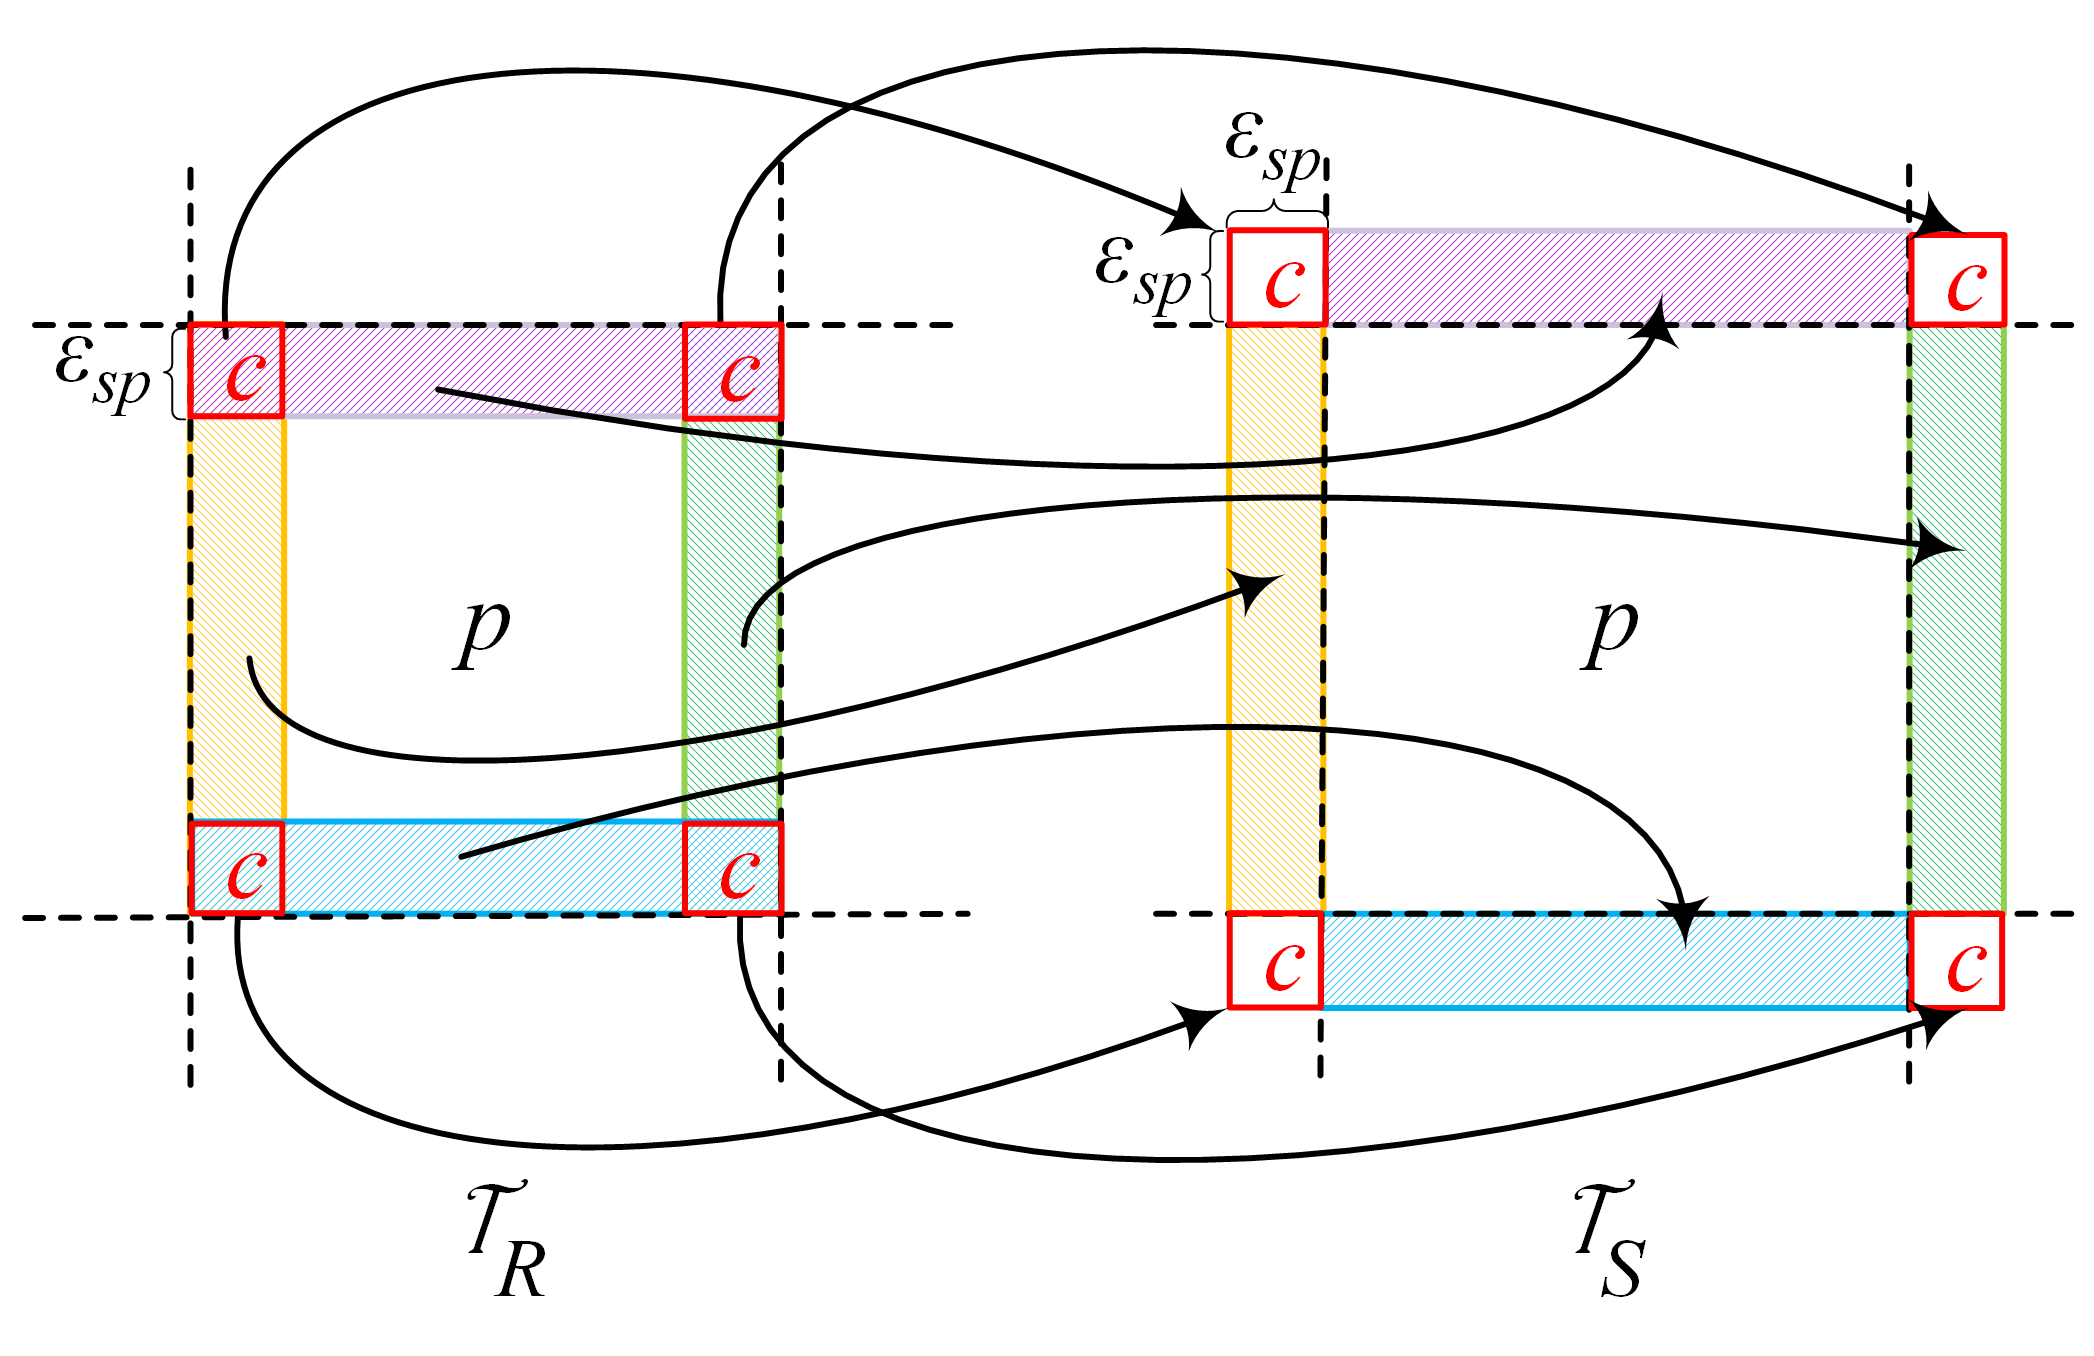
\includegraphics[trim=0 2mm 0 1mm, clip, width=0.34\textwidth]{figures/grid_exchange_slices.png}}
 \vspace{-10pt}
\caption{Blocks in cross-partition search for a partition $p$.}
\label{fig:blocks}
\end{figure}

\let\oldnl\nl% Store \nl in \oldnl
\newcommand{\nonl}{\renewcommand{\nl}{\let\nl\oldnl}}% Remove line number for one line in algorithm

\begin{algorithm}[!ht]
\begin{small}
	\DontPrintSemicolon
	\KwIn{dataset $\mathcal{T}_{R}$, dataset $\mathcal{T}_{S}$, spatial constraint $\epsilon_{sp}$, time series constraint $\epsilon_{ts}$, index method $\mathcal{X}$ (e.g., \btsr or R-tree)}
       \KwOut{Set $Q$ of pairs of geolocated time series satisfying constraints}

	\nonl /* 	{\bf PHASE \#1}: {\em local search per partition} */ \\
	
	$\mathcal{P} \leftarrow$ space partitioning common for both datasets $\mathcal{T}_{R}, \mathcal{T}_{S}$ \\
	$R_{\mathcal{P}} \leftarrow $ distribute $\mathcal{T}_{R}$ and build a local $\mathcal{X}$-index per partition $p \in \mathcal{P}$\\
	$S_{\mathcal{P}} \leftarrow $ distribute $\mathcal{T}_{S}$ and build a local $\mathcal{X}$-index per partition $p \in \mathcal{P}$\\
	\mbox{$L_{\mathcal{P}} \leftarrow \{ ( p , p ): \forall p \in \mathcal{P} \}$} \com*[f]{pairs of identical partitions} \\
	$Q_{\mathcal{P}} \leftarrow blockwiseSimJoin(L_{\mathcal{P}}, R_{\mathcal{P}}, S_{\mathcal{P}},\epsilon_{sp}, \epsilon_{ts})$ \\	
	$storeHDFS(Q_{\mathcal{P}})$  \com*[f]{partial results over partitions} \\

	\nonl /* 	{\bf PHASE \#2a}: {\em cross-partition search in pairs of adjacent bands} */ \\
	
	$\mathcal{B} \leftarrow$ create bands of width $\epsilon_{sp}$ inwards each side of every $p \in \mathcal{P}$ \\
	$R_{\mathcal{B}} \leftarrow $ filter $R_{\mathcal{P}}$ by $\mathcal{B}$ and build a local $\mathcal{X}$-index per band $b \in \mathcal{B}$\\
	$S_{\mathcal{B}} \leftarrow $ filter $S_{\mathcal{P}}$ by $\mathcal{B}$ and build a local $\mathcal{X}$-index per band $b \in \mathcal{B}$\\
	\mbox{$L_{\mathcal{B}} \leftarrow \{ ( r \in R_{\mathcal{B}}, s \in S_{\mathcal{B}}):$ bands $r.b, s.b$ share a side in partitioning $\mathcal{P}\}$} \\
	
%	\mnote{Insert here description of light similarity joins for the optimized method}
	
	$Q_{\mathcal{B}} \leftarrow blockwiseSimJoin(L_{\mathcal{B}}, R_{\mathcal{B}}, S_{\mathcal{B}},\epsilon_{sp}, \epsilon_{ts})$ \\	
	$storeHDFS(Q_{\mathcal{B}})$  \com*[f]{partial results over bands}\\
	
\nonl /* {\bf PHASE \#2b}: {\em cross-partition search in corner-wise pairs of boxes} */ \\
	
	$\mathcal{C} \leftarrow$ create boxes of side $\epsilon_{sp}$ at the corners of each partition $p \in \mathcal{P}$ \\
	$R_{\mathcal{C}} \leftarrow $ filter $R_{\mathcal{P}}$ by $\mathcal{C}$ and build a local $\mathcal{X}$-index per box $c \in \mathcal{C}$\\
	$S_{\mathcal{C}} \leftarrow $ filter $S_{\mathcal{P}}$ by $\mathcal{C}$ and build a local $\mathcal{X}$-index per box $c \in \mathcal{C}$\\
	\mbox{$L_{\mathcal{C}} \leftarrow \{ ( r \in R_{\mathcal{C}}, s \in S_{\mathcal{C}}):$ boxes $r.c, s.c$ share a single corner in  $\mathcal{P}\}$} \\
	$Q_{\mathcal{C}} \leftarrow blockwiseSimJoin(L_{\mathcal{C}}, R_{\mathcal{C}}, S_{\mathcal{C}},\epsilon_{sp}, \epsilon_{ts})$ \\	
	$storeHDFS(Q_{\mathcal{C}})$  \com*[f]{partial results over boxes} \\
			

%%%%%%%%%%%%%%%%%%%%%%%%%%%%%			
\eat{	
	$stripInd \leftarrow calcStripIndices(D_{p})$ \\
	$stripPairs \leftarrow ForwardStripIndices(stripInd.lightBtsrs, stripInd.env, stripInd.extEnv)$ \\
	$candidateMbrPairs \leftarrow GetCandidateMBRs(stripPairs)$ \\
	$stripRes \leftarrow ExecStripJoins(mbrPairs, stripInd.btsrs, \epsilon_{sp}, \epsilon_{ts})$ \\
	$storeHDFS(stripRes)$
}
%%%%%%%%%%%%%%%%%%%%%%%%%%%%%	
	\vspace{6pt}
	\SetKwProg{procTraversal}{Function}{}{}
	\procTraversal{$blockwiseSimJoin(L, R, S, \epsilon_{sp}, \epsilon_{ts})$}{
		$Q \leftarrow \emptyset$ \\		
		\ForEach(\com*[f]{local search}){block pair $(a, b) \in L$}{
		      $\mathcal{I}_{a}^{R} \leftarrow$ local $\mathcal{X}$-index available for dataset ${R}$ in block $a$ \\
		      $\mathcal{I}_{b}^{S} \leftarrow$ local $\mathcal{X}$-index available for dataset ${S}$ in block $b$ \\
			$Q \leftarrow Q \cup SimJoin\mathcal{X}(\mathcal{I}_{a}^{R}.root, \mathcal{I}_{b}^{S}.root, \epsilon_{sp}, \epsilon_{ts})$ \\
		}
		\KwRet $Q$ \com*[f]{results collected from all pairs of blocks}
	}

	\caption{$SimJoinMR(\mathcal{T}_{R},\mathcal{T}_{S}, \epsilon_{sp}, \epsilon_{ts}, \mathcal{X} )$}
	\label{alg:simjoin_mr}
\end{small}
\end{algorithm}


%Once pairs of blocks need be checked at each tier (either $L_{\mathcal{P}}$ for partitions, or $L_{\mathcal{B}}$ for bands, or $L_{\mathcal{C}}$ for boxes), {\em blockwiseSimJoin} (Lines 19-25) takes advantage of the created indices and applies the respective method from Section~\ref{sec:centralized} to return their results.

%Quite importantly, each pair of blocks at any tier can be processed independently of the rest. Hence, for a given partitioning $\mathcal{P}$, once the query is submitted, the required subsets and their indices can be prepared in a {\em distributed} fashion and the respective block-wise checking can be evaluated {\em in parallel} through multiple workers. For a given partition $p$ (first tier), subsets from both datasets (including indices) are assigned to the same worker node. This policy is also applied in the case of bands (or boxes) that need to be checked: the worker responsible for a given partition $p$ receives the data and index concerning objects from the other dataset within an adjacent band (or corner-wise box). %\mnote{{\bf Suppress for brevity?} Further, no exchange of partial results takes place at any stage, so once a worker receives the required block data it can readily process them and issue its own results.} 
%Such processing fits well under the {\em MapReduce} paradigm. In particular, mappers assign data subsets to workers according to  partitioning scheme $\mathcal{P}$. Each worker employs reduce operations to generate the respective indices and store them on HDFS. At query time, a map procedure assigns the indices that reside within each partition to a reducer, which calculates the local results. Simultaneously, mappers shuffle data per block (i.e., band or box) to workers responsible for their neighboring partitions. Finally, a reduce operation is carried out on each pair of such blocks to compute their similarity joins and to store results on HDFS.


Once pairs of blocks need be checked at each tier (either $L_{\mathcal{P}}$ for partitions, or $L_{\mathcal{B}}$ for bands, or $L_{\mathcal{C}}$ for boxes), {\em blockwiseSimJoin} (Lines 19-25) takes advantage of the created indices and applies the respective method from Section~\ref{sec:centralized} to return their results. Each pair of blocks at any tier can be processed independently. Hence, for a given partitioning $\mathcal{P}$, once the query is submitted, the required subsets and their indices can be prepared in a {\em distributed} fashion and the respective block-wise checking can be evaluated {\em in parallel}. For a given partition $p$ (first tier), subsets from both datasets are assigned to the same worker node. This policy is also applied in the case of blocks that need to be checked: the worker responsible for a given partition $p$ receives the data and index concerning objects from the other dataset within an adjacent block. Such processing fits well under the {\em MapReduce} paradigm; mappers assign data subsets to workers according to partitioning scheme $\mathcal{P}$. Each worker employs reduce operations to generate the respective indices and store them on HDFS. At query time, a map procedure assigns the indices that reside within each partition to a reducer, which calculates the local results. Simultaneously, mappers shuffle data per block to workers responsible for their neighboring partitions. Finally, a reduce operation is carried out on each pair of such blocks to compute their similarity joins and to store results on HDFS.


%In terms of MapReduce operations, initially during partitioning, a map procedure assigns the raw geolocated time series to a set of worker nodes according to the partitioning scheme $\mathcal{P}$. The latter then perform reduce operations, generating the respective indices and storing them on the distributed storage. At query time, a map procedure assigns the indices that reside within each cell to a reduce operation, where the local results are calculated and stored. Simultaneously, two map procedures assign raw geolocated time series contained within each band and box to a set of worker nodes, after properly grouping the bands that share a common side and boxes that share a common corner on the selected partitioning. Finally, a reduce procedure occurs on the grouped geolocated time series, performing the corresponding similarity joins and storing the band and box results on the distributed storage.

Overall, this method manages to provide correct and complete results for any similarity join query over two datasets of geolocated time series. This is stated in the following:
\begin{mylemma}
Algorithm~\ref{alg:simjoin_mr} issues all qualifying results of similarity join between two datasets $\mathcal{T}_{R}$, $\mathcal{T}_{S}$ of geolocated time series, without probing candidate pairs more than once and without any false misses.
\end{mylemma}
\vspace{-3mm}
\begin{proof} Regarding {\em correctness}, consider a given partition $p \in \mathcal{P}$, as depicted in Figure~\ref{fig:blocks} and let $R_{p}$ be the objects of $\mathcal{T}_{R}$ having their location contained therein. Obviously, any of their possibly qualifying pairs from dataset $\mathcal{T}_{S}$ must be within distance $\epsilon_{sp}$. So, it suffices to examine similarity between objects in $R_{p}$ with those objects of $\mathcal{T}_{S}$ topologically located within a {\em buffer} that expands partition $p$ by distance $\epsilon_{sp}$. Clearly, the area covered by the nine blocks (one partition, four bands, and four boxes) concerning $\mathcal{T}_{S}$ is exactly this buffer zone, so $Q_{cand}(p) = \{ (T_{R}, T_{S} ): within(T_{R}.loc, p), within(T_{S}.loc, buffer(p, \epsilon_{sp})) \}$ provides all possible candidates in a given partition $p$. As partitions hold disjoint subsets of the raw data, iterating with the same logic over each partition $p \in \mathcal{P}$, confirms that all candidates are examined. 

Regarding {\em completeness}, observe that the pairs of blocks involved at each stage include all possible candidates to probe from each dataset. At the first tier, searching in each partition $p$ (common for either dataset) provides all qualifying pairs having their constituent objects both located in $p$. Cross-searching beyond the boundary of each partition $p$ is meaningful only along the adjacent bands and boxes, each of them coming from a distinct neighboring partition to $p$. Clearly, in each of those nine blocks, a disjoint subset of candidate pairs from the two datasets is examined and their union is $Q_{cand}(p)$. Hence, each candidate pair is probed only once, and no qualifying results can ever be missing from the final answer.
\end{proof}


\subsubsection{Minimizing Data Shuffling}
\label{subsec:optimized}

Recall that a worker $w$ already has locally available all data for subsets of $\mathcal{T}_{R}, \mathcal{T}_{S}$ located in its assigned partition $p$. This is sufficient for its own local search, but $w$ still needs to send raw data concerning its four bands and four boxes for the cross-partition search.

%This is sufficient for the first phase only, so this worker needs to get extra information from other workers holding subsets of $\mathcal{T}_{R}$ over its neighboring partitions so as to provide complete results. For the second phase, it must get subsets of $\mathcal{T}_{R}$ concerning its four adjacent bands and its four corner-wise-aligned boxes, as depicted in Figure~\ref{fig:blocks}. In addition, worker $w$ must prepare subsets of its local chunk of $\mathcal{T}_{S}$ concerning its own bands and boxes to be compared against those received from its neighbors. Finally, worker $w$ must built indices for each such subset so as to facilitate similarity join search between pairs of such blocks.

%Instead of transferring chunks of raw data from one worker to another, which may incur considerable communication cost, 

%This evaluation strategy can be further optimized by minimizing the amount of data that needs to be shuffled during cross-partition search. We introduce an intermediate filtering step that takes advantage of the pruning power of our \btsr index. More concretely, consider a given block (band or box) $a$ over dataset $\mathcal{T}_{R}$ held in worker $w'$ that must be shipped to worker $w$ responsible for partition $p$. Instead, $w'$ builds a \btsr $\mathcal{I}_{a}^{R}$ over this subset in $a$, and sends this index only to worker $w$, which builds its own \btsr $\mathcal{I}_{b}^{S}$ over its local subset of $\mathcal{T}_{S}$ within its corresponding block $b$. Checking for similarity joins against those two indices can be carried out with Algorithm~\ref{alg:sim_joins_btsr}. This returns pairs $\{ (mbr^{a}_{i}, mbr^{b}_{j}) \}$ of overlapping MBRs, where $mbr^{a}_{i}$ is an MBR over block $a$ and $mbr^{b}_{j}$ is over block $b$, and each one contains candidate objects for refinement. The list $\{ mbr^{a}_{i} \}$ of all identified  MBRs concerning block $a$ is returned to worker $w'$ and the raw geolocated time series within each such MBR can be readily accessed thanks to the already available \btsr $\mathcal{I}_{a}^{R}$. Those MBR-filtered time series are then shipped to worker $w$, which also retrieves its own raw data from \btsr $\mathcal{I}_{b}^{S}$ concerning those MBRs $\{ mbr^{b}_{j} \}$ identified for its own block $b$. Finally, those two MBR-filtered subsets of geolocated time series are each indexed with a new {\btsr} and joined according to the similarity criteria to yield their matching results. As confirmed in our empirical tests, this index-guided shuffling can reduce the raw data transferred between workers by more than 50\% without sacrificing performance.

This evaluation strategy can be further optimized by minimizing the amount of data that needs to be shuffled during cross-partition search. We introduce an intermediate filtering step that takes advantage of the pruning power of our \btsr index. Consider a given block $a$ over dataset $\mathcal{T}_{R}$ held in worker $w'$ that must be shipped to worker $w$ responsible for partition $p$. Instead, $w'$ builds a \btsr $\mathcal{I}_{a}^{R}$ over this subset in $a$, and sends this index only to worker $w$, which builds its own \btsr $\mathcal{I}_{b}^{S}$ over its local subset of $\mathcal{T}_{S}$ within its corresponding block $b$. Checking for similarity joins against those two indices can be carried out with Algorithm~\ref{alg:sim_joins_btsr}. This returns pairs $\{ (mbr^{a}_{i}, mbr^{b}_{j}) \}$ of overlapping MBRs, where $mbr^{a}_{i}$ is an MBR over block $a$ and $mbr^{b}_{j}$ is over block $b$, and each one contains candidate objects for refinement. The list $\{ mbr^{a}_{i} \}$ of all identified  MBRs concerning block $a$ is returned to worker $w'$ and the raw geolocated time series within each such MBR can be readily accessed thanks to the already available \btsr $\mathcal{I}_{a}^{R}$. Those MBR-filtered time series are then shipped to worker $w$, which also retrieves its own raw data from \btsr $\mathcal{I}_{b}^{S}$ concerning those MBRs $\{ mbr^{b}_{j} \}$ identified for its own block $b$. Finally, those two MBR-filtered subsets of geolocated time series are each indexed with a new {\btsr} and joined according to the similarity criteria to yield their matching results. As confirmed in our empirical tests, this index-guided shuffling can reduce the raw data transferred between workers by more than 50\% without sacrificing performance.